\chapter{三角学}
\label{ch:Trigonometry}
还是一样,和IGCSE阶段相比,在Alevel阶段我们将了解更多关于三角比的以及三角函数的内容

\section*{学习目标}
\begin{todolist}
	\item 牢记并应用特殊角的正弦值,余弦值,正切值。以及相关变化
	\item 牢记并运用三角恒等式
	\item 求算给定区间区间内的含有三角比的方程
	\item 理解单位圆的作用
	\item 绘制$\sin$,$\cos$,$\tan$的函数图像,包括改变振幅,周期,初相位等变化
	\item 理解反三角函数可以用来求算角的大小
\end{todolist}
\clearpage

\section{三角比}
\label{sec:Trigonometric Ratio}
回顾一下三角比的定义 SOH CAH TOA\footnote{Opposite, Adjacement, Hypotenuse的缩写,sine,cosine和tangent的缩写}。

\subsection*{特殊角的三角比}
\label{subsec:Special Angle}
结合两个特殊三角形。可以完成以下的表格
\begin{figure}[H]
\centering
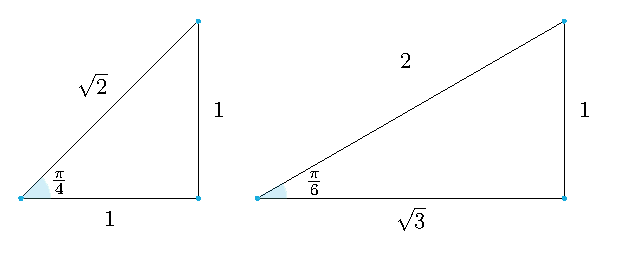
\includegraphics[width=0.8\textwidth]{SpecialTriangle}
\caption{两个特殊三角形以及边长}
\end{figure}

\begin{table}[H]
\centering
\begin{tblr}{|l|c|c|c|}
\hline
$\theta$ & $\frac{\pi}{6}$ & $\frac{\pi}{4}$ & $\frac{\pi}{3}$\\
\hline
$\sin\theta$ &$\frac{1}{2}$& & \\
\hline
$\cos\theta$ & & $\frac{\sqrt2}{2}$& \\
\hline
$\tan\theta$ & $\frac{\sqrt3}{3}$ & & \\
\hline
\end{tblr}
\end{table}

\begin{TaskBox}
完成上方表格当中剩余的空白处
\end{TaskBox}


\subsection*{单位圆}
\label{subsec:Unit Circle}
当我们引入半径为$1$,圆心在原点的圆的时候,构造任意的半径旋转的角度$\theta$就可以用旋转点的\emph{横}
/\emph{纵}坐标来代替该角度$\theta$的正余弦值,以及求算正切值。如下图:

\begin{figure}[H]
\centering
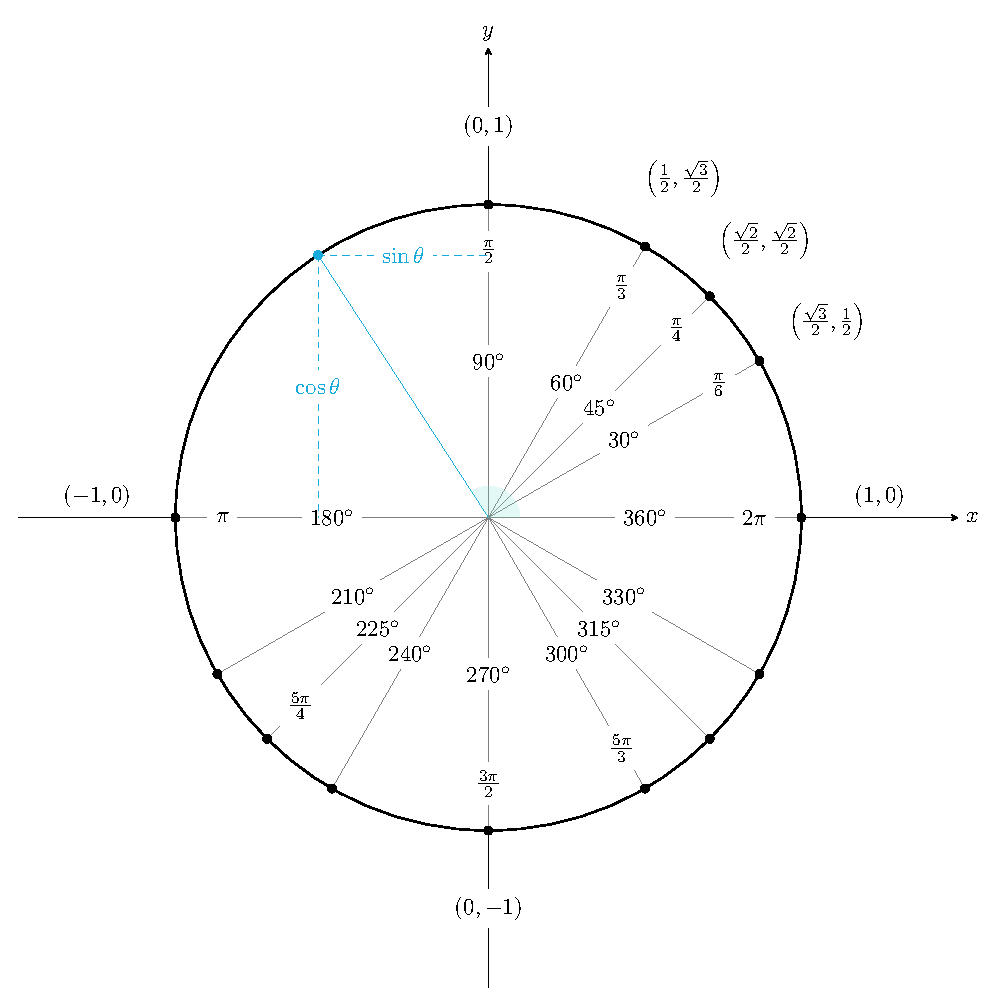
\includegraphics[width=0.8\textwidth]{unitcircle}
\caption{单位圆用点的坐标表示一个角度的$\sin$,$\cos$值}
\end{figure}

\begin{TaskBox}
补齐单位圆上剩余的特殊点的坐标,以及确定对应角度的正弦,余弦,正切值。
\end{TaskBox}

\subsection*{三角恒等式}
\label{subsec:Trig Identity}
根据单位圆上或者其他的证明,有以下的恒等关系始终存在,这些恒等关系需要牢记并进行运用
\begin{align}
\sin^2\theta+\cos^2\theta &= 1\\
\sin(\frac{\pi}{2}-\theta) &= \cos \theta \\
\tan \theta =\frac{\sin \theta}{\cos \theta}
\end{align}

\begin{TaskBox}
已知某角度$\theta$的$\tan$值为3;求算$\sin \theta$ 和$\cos \theta$。
\end{TaskBox}
\clearpage


\section{三角函数}
\label{sec:Unit Circle and Trigonometric Function}
由于单位圆的存在,我们在理解角度上的时候,再也不需要拘泥于度数制的限制,$\theta$角可以取任意的值,并且,由于负值的时候,仅需要把角度进行顺时针旋转即可。因此以角度$\theta$作为自变量$x$,以其三角比的值作为因变量$y$。构建如下的三种函数关系$y=\sin x$, $y=\cos x$, $y=\tan x$。逐一进行研究

\subsection*{正弦函数}
\label{subsec:Sine function}
我们将采用描点法绘制三种函数的图像,首先,结合单位圆,完成以下的表格:

\begin{table}[H] %这个表格的长宽设计的不太合理。
\centering
\begin{tblr}{
	colspec={|l|[2pt]c|c|c|c|c|c|c|c|c|},
	hspan=even, %设置一样长度
	vspan=even,
	}
\hline 
$x$(in rad) & 0 & $\frac{\pi}{6}$ & $\frac{\pi}{4}$ & $\frac{\pi}{3}$ & $\frac{\pi}{2}$ &$\frac{2\pi}{3}$ & $\frac{3\pi}{4}$&$\frac{5\pi}{6}$ &$\pi$\\
\hline
$y=\sin x$ &$\quad$ &$\quad$ &$\quad$ &$\quad$ &$\quad$ &$\quad$ &$\quad$ &$\quad$ \\
\hline
$x$(in rad)& $\frac{7\pi}{6}$ & $\frac{5\pi}{4}$ & $\frac{4\pi}{3}$& $\frac{3\pi}{2}$ & $\frac{10\pi}{6}$& $\frac{7\pi}{4}$& $\frac{11\pi}{6}$ &$2\pi$\\
\hline
$y=\sin x$ &$\quad$ &$\quad$ &$\quad$ &$\quad$ &$\quad$ &$\quad$ &$\quad$ &$\quad$ \\
\hline
\end{tblr}
\end{table}

\begin{TaskBox}
完成以上的表格
\tcblower
在下方的函数图像中选择对应的点
\end{TaskBox}

\begin{figure}[H]
\centering
\includegraphics[width=\textwidth]{sinefunc}
\caption{标准正弦函数图}
\end{figure}

因此就形成正弦函数的图像。请关注以下的几个点:
\begin{itemize}
	\item 函数最大值和最小值出现的地方
	\item 函数值为0的地方
	\item 该函数的周期性
	\item 该函数的对称性
\end{itemize}

\subsection*{余弦函数}
\label{subsec:Cosine Function}
一样的过程,再重复一遍。

\begin{table}[H]
\centering
\begin{tblr}{
	colspec={|l|[2pt]c|c|c|c|c|c|c|c|c|},
	hspan=even, %设置一样长度
	vspan=even,
	}
\hline 
$x$(in rad) & 0 & $\frac{\pi}{6}$ & $\frac{\pi}{4}$ & $\frac{\pi}{3}$ & $\frac{\pi}{2}$ &$\frac{2\pi}{3}$ & $\frac{3\pi}{4}$&$\frac{5\pi}{6}$ &$\pi$\\
\hline
$y=\cos x$ &$\quad$ &$\quad$ &$\quad$ &$\quad$ &$\quad$ &$\quad$ &$\quad$ &$\quad$ \\
\hline
$x$(in rad)& $\frac{7\pi}{6}$ & $\frac{5\pi}{4}$ & $\frac{4\pi}{3}$& $\frac{3\pi}{2}$ & $\frac{10\pi}{6}$& $\frac{7\pi}{4}$& $\frac{11\pi}{6}$ &$2\pi$\\
\hline
$y=\cos x$ &$\quad$ &$\quad$ &$\quad$ &$\quad$ &$\quad$ &$\quad$ &$\quad$ &$\quad$ \\
\hline
\end{tblr}
\end{table}

绘制的函数图如下:
\begin{figure}[H]
\centering
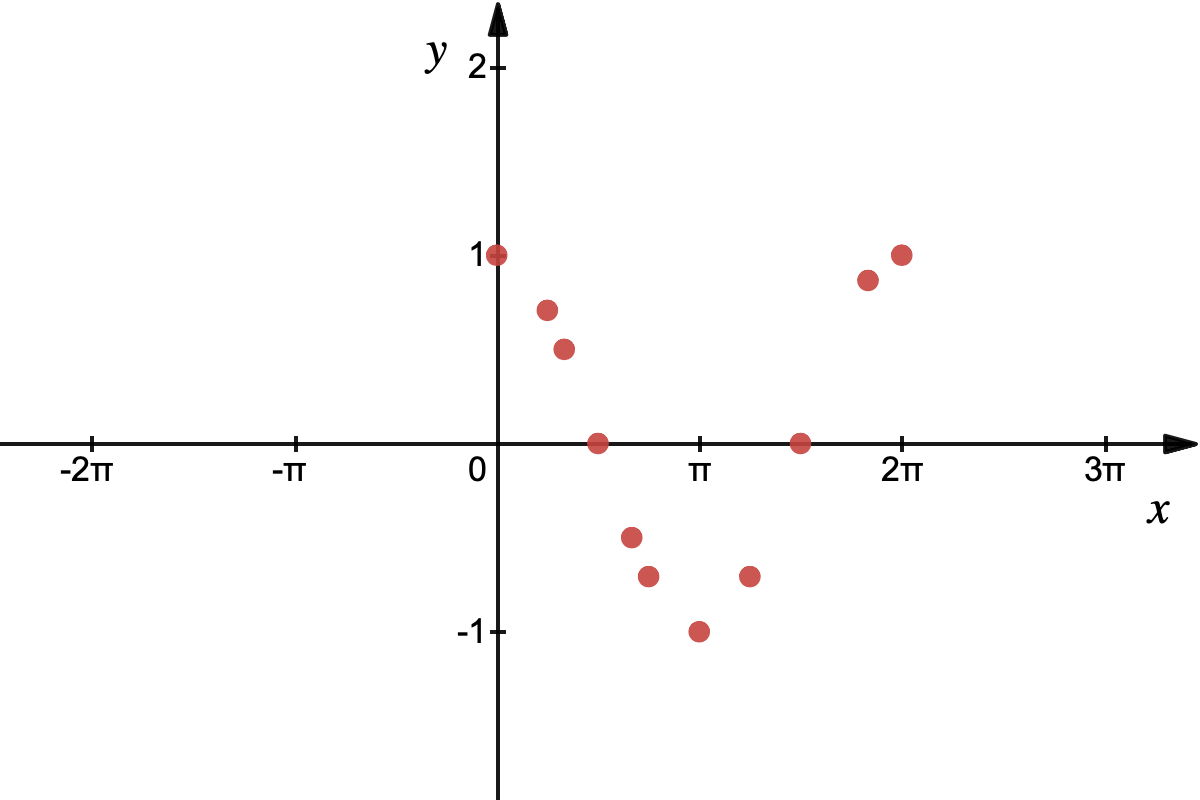
\includegraphics[width=\textwidth]{cosinefunc}
\caption{标准余弦函数图}
\end{figure}

\begin{TaskBox}
根据描点,绘制$y=cos(x)$的函数图像,并且绘制小于0,以及大于$2\pi$时的图像。
\end{TaskBox}

与正弦函数一样,请描述这个图像的一下几个方面:
\begin{itemize}
	\item 函数最大值和最小值出现的地方
	\item 函数值为0的地方
	\item 该函数的周期性
	\item 该函数的对称性
\end{itemize}


\subsection*{正切函数}
\label{subsec:Tangent Function}
根据$\tan x =\frac{\sin x}{\cos x}$。完成以下的表格的绘制:

\begin{table}[H]
\centering
\begin{tblr}{
	colspec={|l|[2pt]c|c|c|c|c|c|c|c|c|},
	hspan=even, %设置一样长度
	vspan=even,
	}
\hline 
$x$(in rad) & 0 & $\frac{\pi}{6}$ & $\frac{\pi}{4}$ & $\frac{\pi}{3}$ & $\frac{\pi}{2}$ & $-\frac{\pi}{6}$ & -$\frac{\pi}{4}$ & -$\frac{\pi}{3}$ & -$\frac{\pi}{2}$\\
\hline
$y=\tan x$ &$\quad$ &$\quad$ &$\quad$ &$\quad$ &$\quad$ &$\quad$ &$\quad$ &$\quad$
\hline
\end{tblr}
\end{table}

因此该函数的图像如下图:
\begin{figure}[H]
\centering
\includegraphics[width=\textwidth]{tangfunc}
\caption{标准正切函数}
\end{figure}

\noindent 有两个点是额外值得关注的,\\
第一个是$y=\tan x$的周期此时不是$2\pi$。应该变成了多少?\\
第二个是\gls{asymptote}。由于$x$不能取得$\frac{\pi}{2}$以及其整倍数值,因此函数的图像不可能与$x=\frac{\pi}{2}$相交,只能无限地靠近该竖直直线,因此是有渐近线的。这是正切函数独有的

\begin{SummBox}
三种基础的三角函数图像分别如下图:
\begin{figure}[H]
\centering
\includegraphics[width=0.3\textwidth]{sinefunc-2}
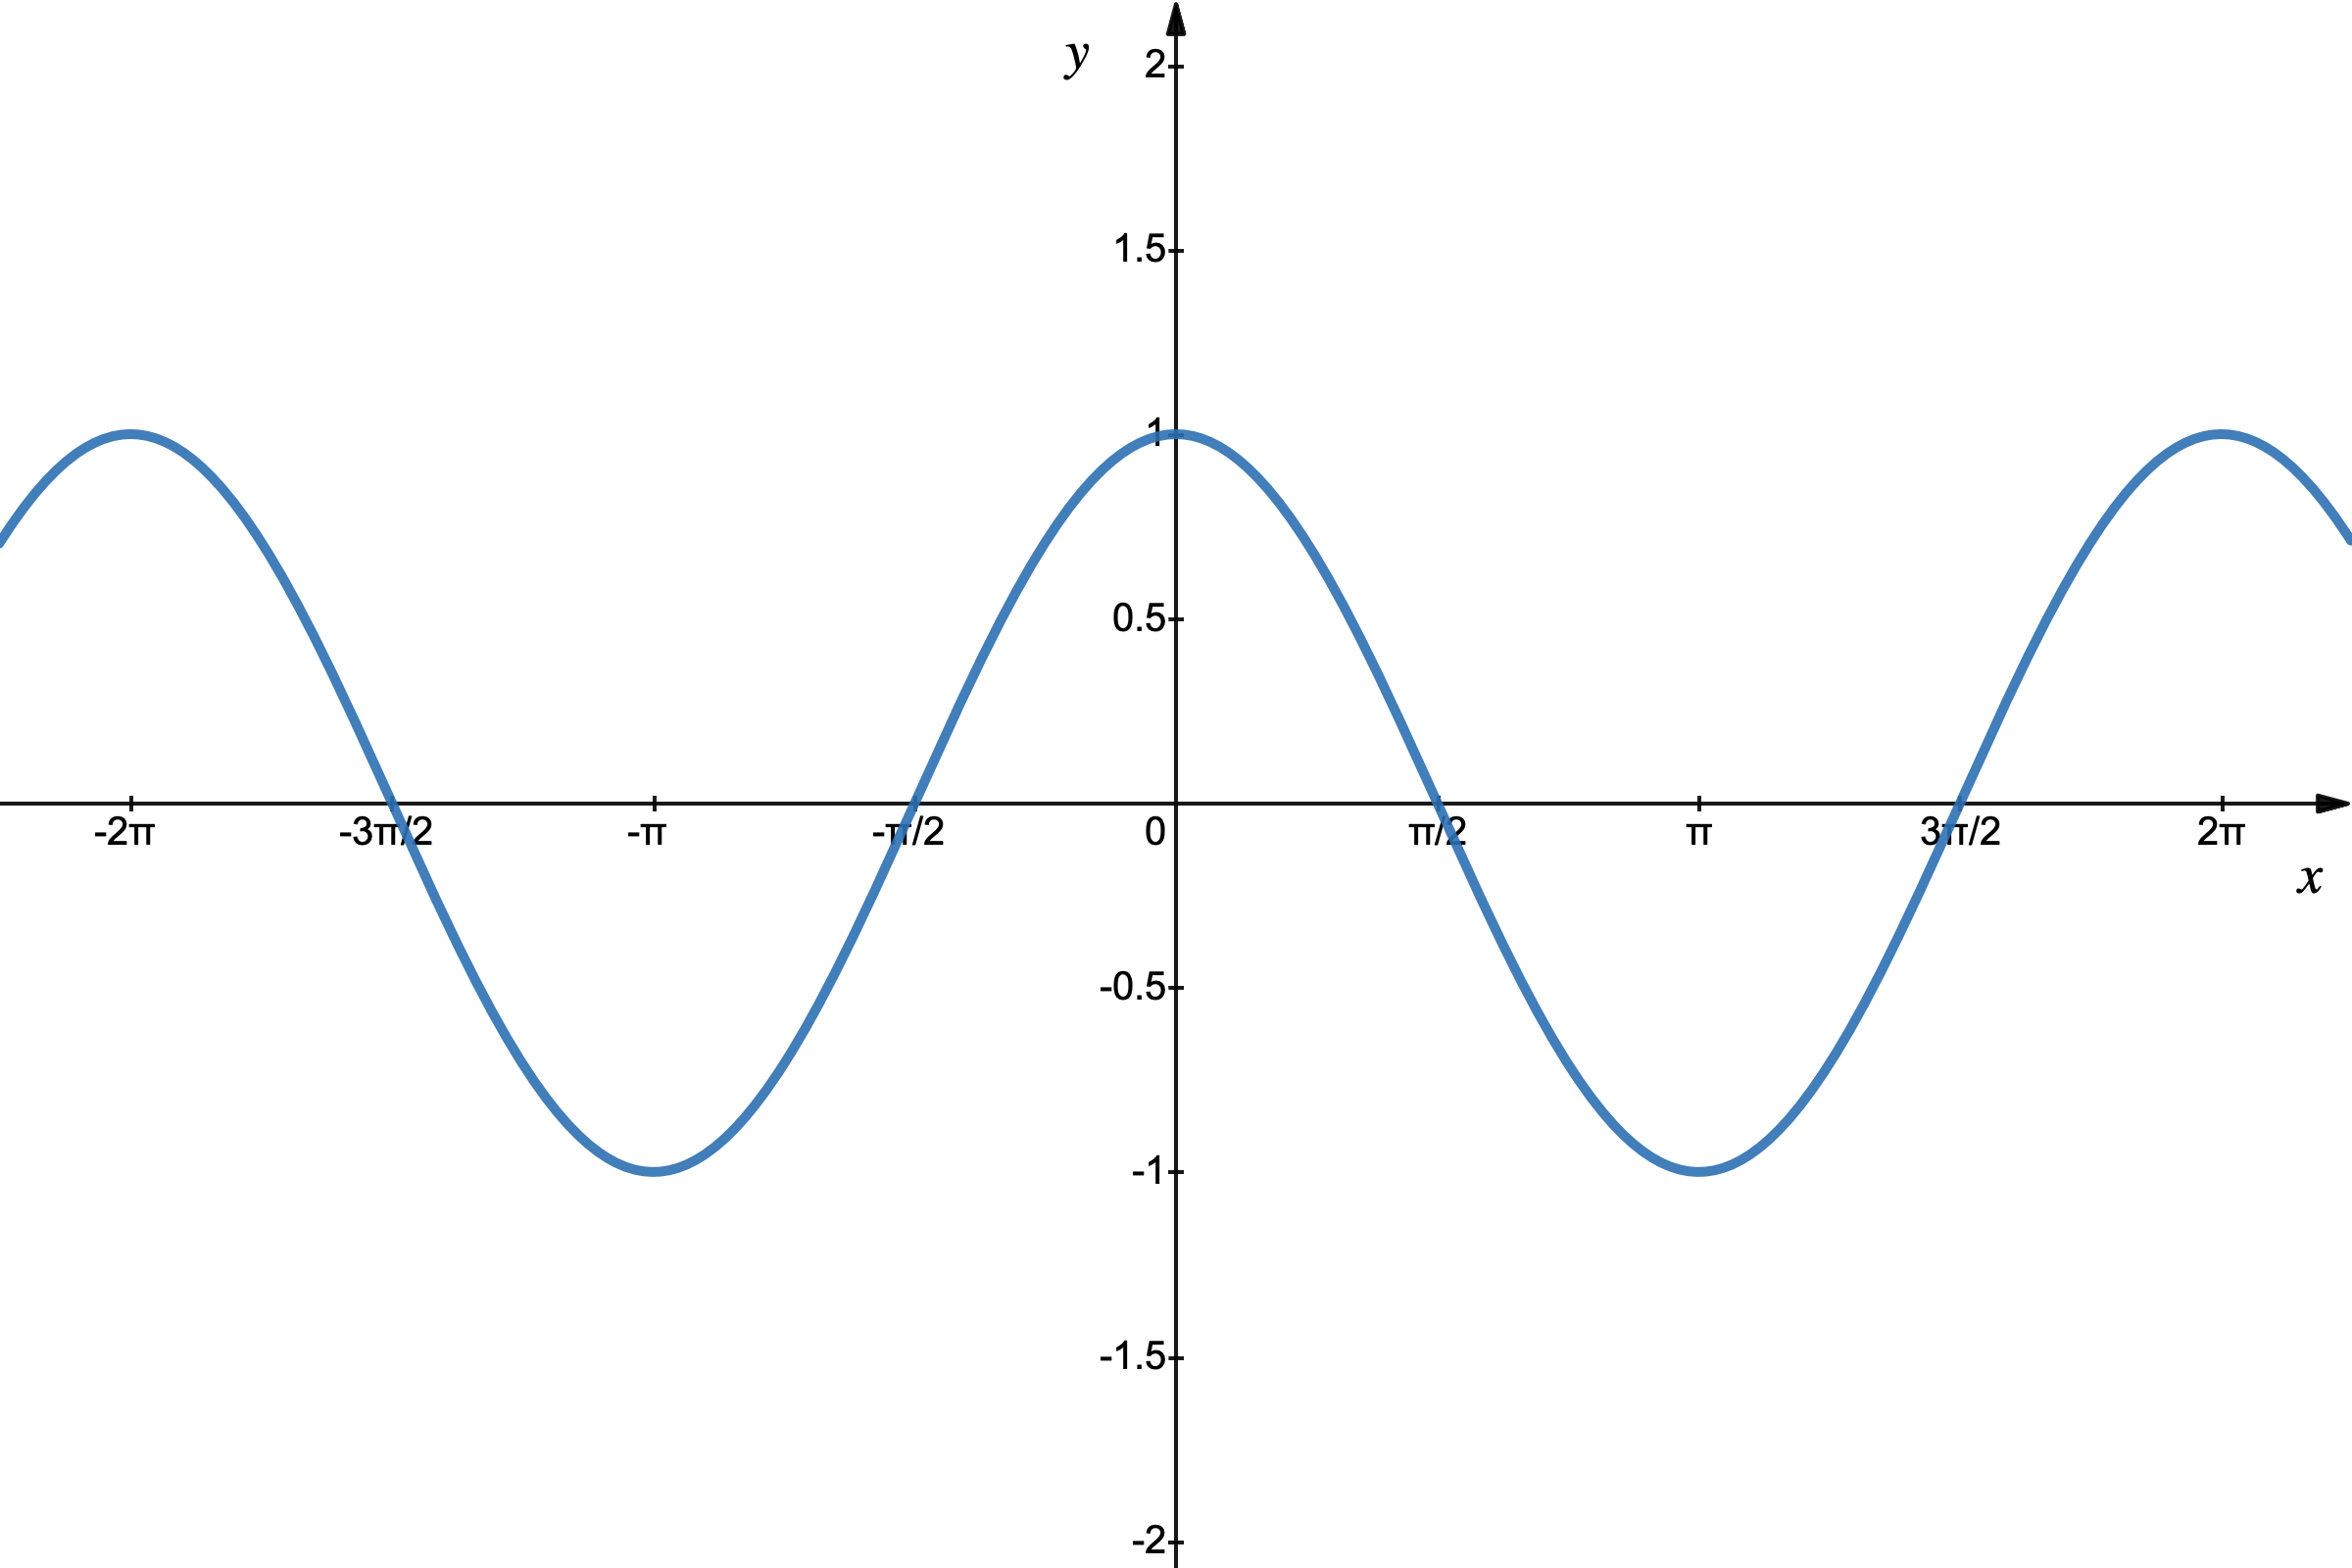
\includegraphics[width=0.3\textwidth]{cosinefunc-2}
\includegraphics[width=0.3\textwidth]{tangfunc-2}
\end{figure}
需要牢记特殊点(5个)。
\end{SummBox}


\subsection*{非标准三角函数}
\label{subsec:Nonstandard Trigonometric Function}
回顾一下之前我们所说的函数的变形。这一小节的内容就是\emph{上加下减,左加右减}以及\emph{拉伸压缩}的具体应用。

因此,我们需要解决如下的几种变形,以及这三者之间的结合。最终实现绘制$y=A\sin (\omega x+\varphi)+C$的图像。

\subsubsection*{水平相位}
$y=\sin (x+\varphi)$会产生水平方向的移动。利用左加右减即可。
\begin{TaskBox}
在下图$y=\sin x$的函数图像中,绘制$y=\sin(x+\frac{\pi}{6})$ 以及 $y=\sin(x-\frac{\pi}{4})$的图像。
\begin{figure}[H]
\centering
\includegraphics[width=0.8\textwidth]{sinefunc-2}
\end{figure}

\end{TaskBox}


\subsubsection*{中间值的移动}
$y=\sin x +C$会产生竖直方向的移动。利用上加下减即可。
\begin{TaskBox}
在下图$y=\sin x$的函数图像中,绘制$y=\sin x+1$ 以及 $y=\sin x-2$的图像。
\begin{figure}[H]
\centering
\includegraphics[width=0.8\textwidth]{sinefunc-2}
\end{figure}
\end{TaskBox}

\subsubsection*{最值的拉伸与翻折}
$y=A\sin x$ 会使的图像发生拉伸变形\\
当$A>1$时,竖直方向上的拉长,会使得函数的最值从$\pm 1$变成 $A\cdot \pm 1=\pm A$;\\
当$0<A<1$时,则是将函数压扁。\\
如果$A$是负值,只需要在拉伸或者压缩之后再沿着$x$轴进行翻折即可。
、
\begin{TaskBox}
在下图$y=\sin x$的函数图像中,绘制$y=-3\sin x$ 以及 $y=\frac{1}{2}\sin x$的图像。
\begin{figure}[H]
\centering
\includegraphics[width=0.8\textwidth]{sinefunc-2}
\end{figure}
\end{TaskBox}

\subsubsection*{周期的变化}
$y=\sin(\omega x)$会产生水平方向的拉伸或者压缩。因此:\\
当$\omega>1$时,将整个图像做压缩,周期会变成$\frac{2\pi}{\omega}$\\
当$0<\omega<1$时,将整个图像做拉伸,周期会变成$\frac{2\pi}{\omega}$\\

\begin{TaskBox}
在下图$y=\sin x$的函数图像中,绘制$y=\sin (4x)$ 以及 $y=\sin (\frac{1}{2}x)$的图像。
\begin{figure}[H]
\centering
\includegraphics[width=0.8\textwidth]{sinefunc-2}
\end{figure}
\end{TaskBox}
\clearpage

\section{反三角}
\label{sec:Inverse Trig}
既然角度有对应的三角比值,那么根据三角比值也能反推角度。此时我们只需要利用\gls{inverse trig}

\subsection*{反三角函数的定义}
举例:$\sin \frac{\pi}{6}= \frac{1}{2}$。因此当已知一个角的sine值为$\frac{1}{2}$时,该角度可以通过$\sin^{-1} (\frac{1}{2})$或者$\arcsin \left( \frac{1}{2}\right)$确定
如下图所示
\begin{figure}[H]
\centering
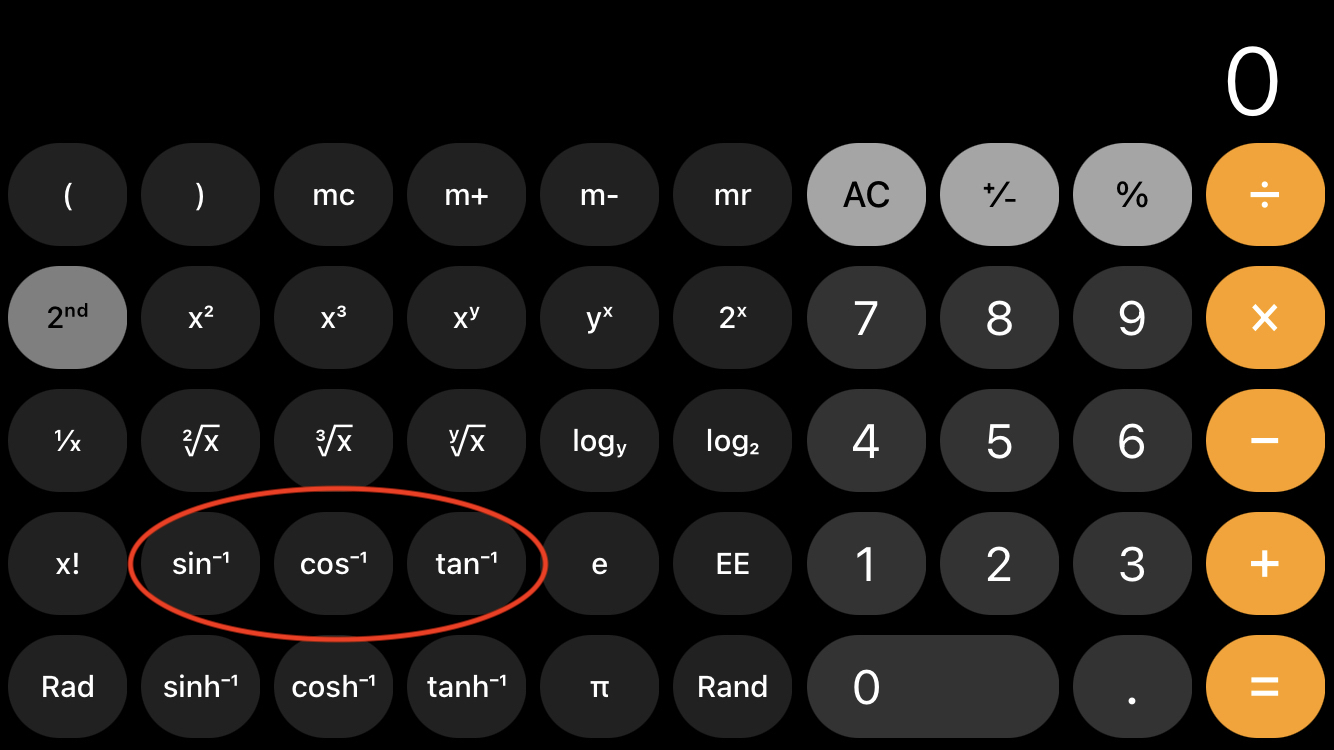
\includegraphics[width=0.7\textwidth]{ioscalc}
\caption{iPhone上如何调出这个反三角函功能?}
\end{figure}

\subsection*{求解$\sin x=a$的结果}
利用刚才所说:
$x=\sin^{-1} a=\theta$。但是,如果我们将$x$的范围限制在$0\le x\le 2\pi$的话。这样的解会有两个,可以利用单位圆进行确定。
\begin{figure}[H]
\centering
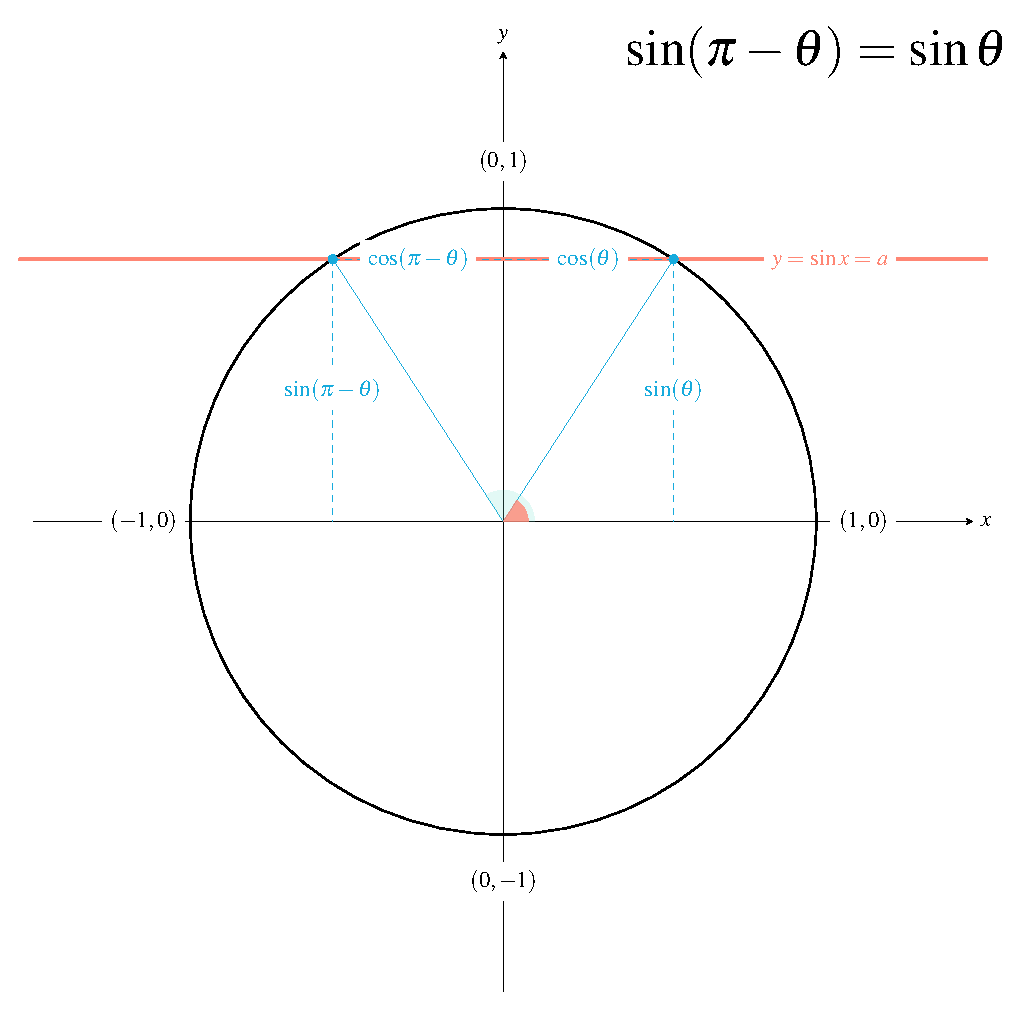
\includegraphics[width=0.5\textwidth]{sina}
\caption{利用单位圆求解$\sin x=a$}
\end{figure}

因此,在一个周期的图像内,一般而言有两个角度的正弦值,可以等于同样的结果,两者之和为$\pi$ 或者 180\si{\degree}。 比如$\sin \frac{\pi}{6}=\sin \frac{5\pi}{6}=\frac{1}{2}$。


\subsection*{求解$\cos x=a$的结果}
和刚才一样。$x=\cos^{-1} a=\theta$。但是,如果我们将x的范围限制在$0\le x\le 2\pi$的话。这样的解也会有两个。
\begin{figure}[H]
\centering
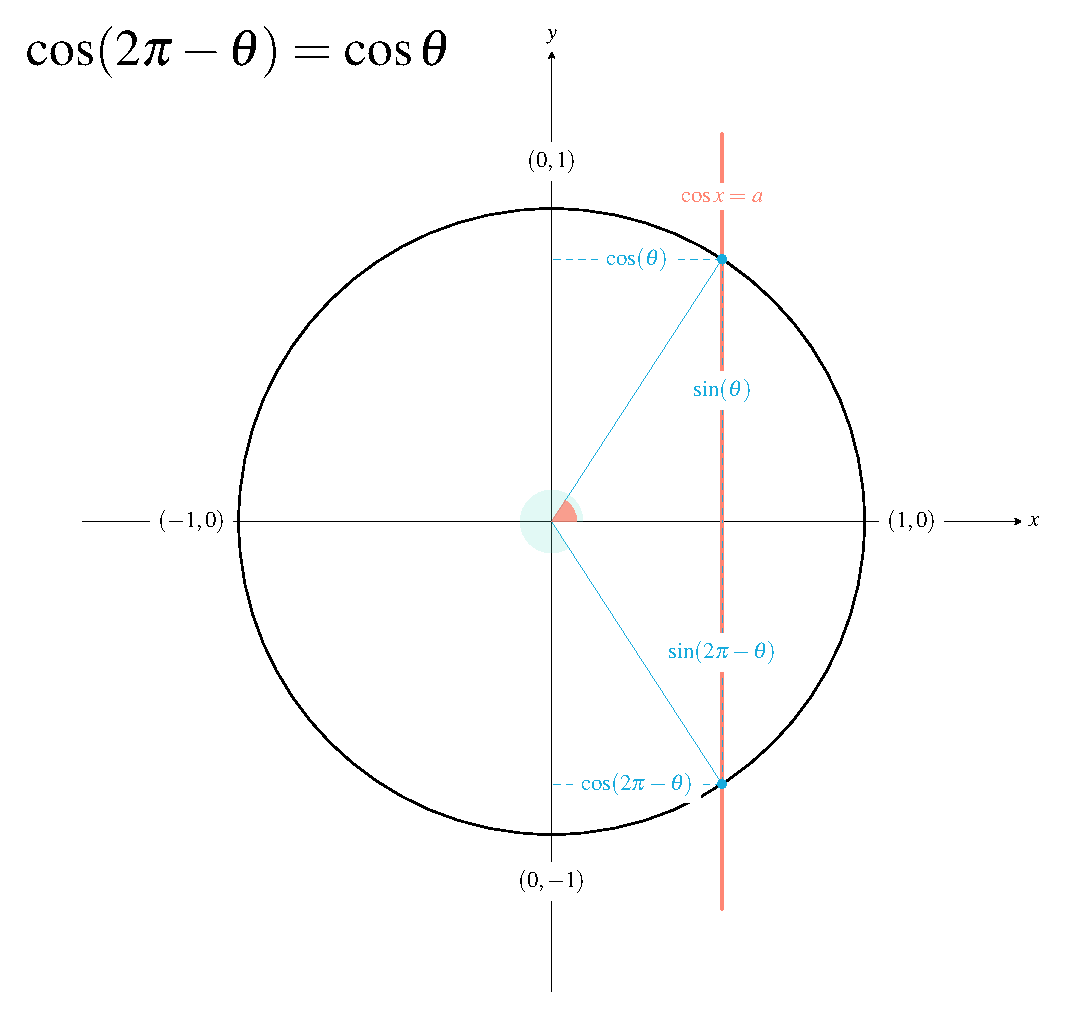
\includegraphics[width=0.5\textwidth]{cosa}
\caption{利用单位圆求解$\cos x=a$}
\end{figure}
因此,在一个周期的图像内,一般而言有两个角度的余弦值,可以等于同样的值,两者之和为$2\pi$ 或者 $360$\si{\degree}。比如$\cos \frac{\pi}{3}=\cos \frac{5\pi}{3}=\frac{1}{2}$。


\subsection*{求解$\tan x=a$的结果}
和刚才一样。$x=\tan^{-1} a=\theta$。但是,如果我们将$x$的范围限制在$0\le x\le 2\pi$的话。这样的解也会有两个。

\begin{figure}[H]
\centering
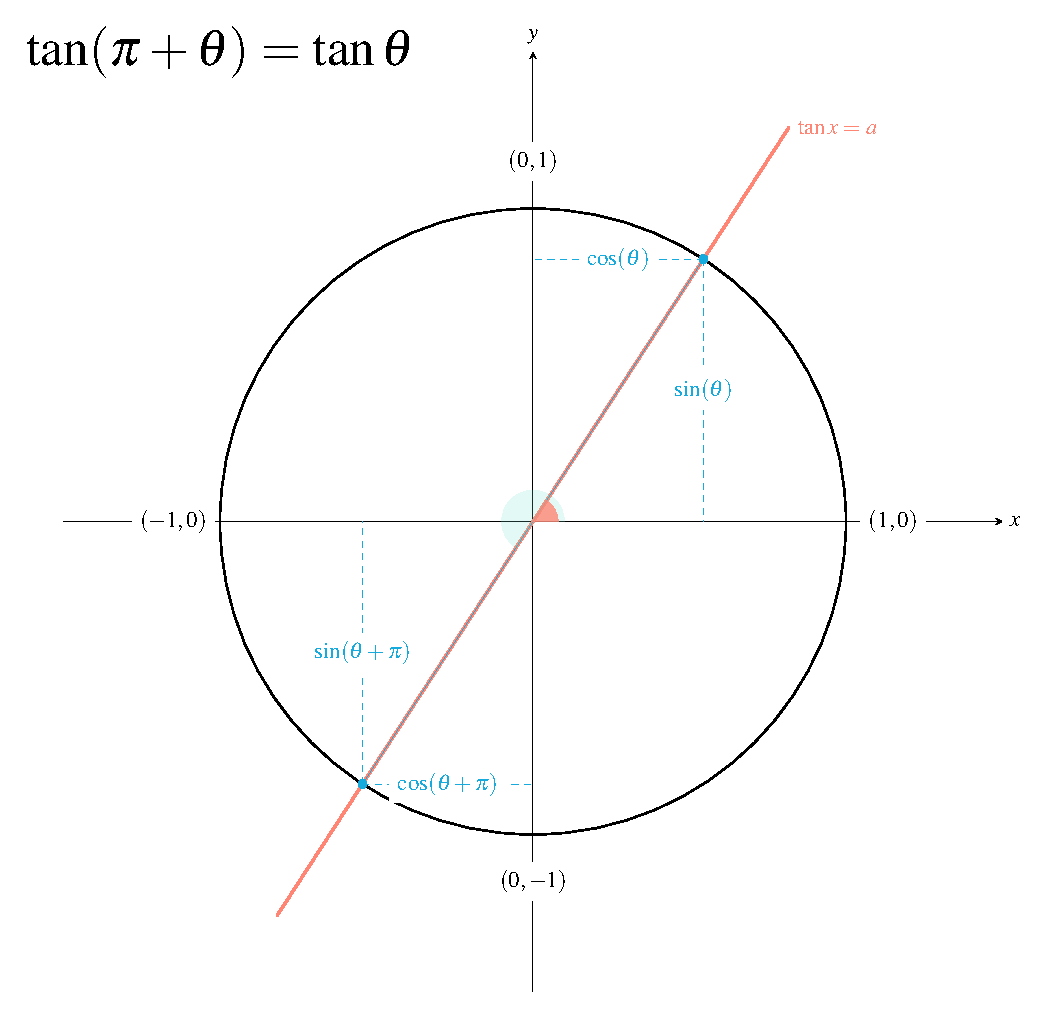
\includegraphics[width=0.5\textwidth]{tana}
\caption{利用单位圆求解$\tan x=a$}
\end{figure}
因此,在两个周期的图像内,一般而言有两个角度的正切值,可以等于同样的值,两者之差为$\pi$ 或者 $180$\si{\degree}。比如$\tan \frac{\pi}{4}=\tan \frac{5\pi}{4}=1$。

\begin{SummBox}
1.如果两个角$\alpha$和$\beta$,满足$\alpha+\beta=\pi$,那么$\sin \alpha=\sin \beta$;\\
2.如果两个角$\alpha$和$\beta$,满足$\alpha+\beta=2\pi$,那么$\cos \alpha=\cos \beta$;\\
3.如果两个角$\alpha$和$\beta$,满足$\alpha-\beta=\pi$,那么$\tan \alpha=\tan \beta$;
\end{SummBox}

\begin{TaskBox}
以上的总结内容仅针对于$[0,2\pi)$,但是由于周期性的存在,两角相等的结果还有其他的结论。尝试推导,当$-\pi\le x\le \pi$时,$\alpha$和$\beta$需要满足什么条件才可以使其正弦值相等。
\end{TaskBox}

\clearpage

\section{含有三角函数的方程}
\label{sec:Equation with Trig}
现在开始处理含有的三角比的方程。
\begin{ExampleBox}
$3\sin(2x)+1 =0$ for $-\pi\le x\le \pi$\\

Solution:
\begin{align*}
\sin (2x) &= -\frac{1}{3}\\
		2x &=\sin^{-1}\left(-\frac{1}{3}\right)\\
		   &=-0.340 \quad \text{or} \quad  =\pi-(-0.340)\\
 		x  &= -0.170 \quad \text{or} \quad -1.400
\end{align*}

参考如下图:
\begin{figure}[H]
\centering
\includegraphics[width=0.5\textwidth]{solvetrig}
\caption{利用正弦图像确定$2x$两个值的对应关系}
\end{figure}
\end{ExampleBox}

再看一个例子:
\begin{ExampleBox}
$3 \sin^2\theta - 5 \cos\theta - 1 = 0$ for $0\si{\degree}\le \theta\le 360\si{\degree}$\\
\tcblower
Solution:

首先,要尽可能地将方程当中只包含一个三角比,在这里需要利用三角恒等式$\sin^2\theta +\cos^2\theta =1$进行化简,整理得到:
\begin{align*}
3(1-\cos^2\theta) -5\cos\theta -1 &= 0\\
-3\cos^2\theta -5\cos\theta +2 &=0\\
3\cos^2\theta +5\cos\theta -2 &=0\\
(3\cos\theta -1)(\cos\theta +2) &=0\\
\cos \theta =\frac{1}{3} &\text{ or } \cos \theta =-2 \quad \text{impossible, thus ignored}\\
\theta &=\cos^{-1}(\frac{1}{3})\\
\theta &=70.53\si{\degree} \text{ or } 360\si{\degree}-70.53\\
		&=70.53\si{\degree} \text{ or }  289.47\si{\degree}
\end{align*}
如图像所示:
\begin{figure}[H]
\centering
\includegraphics[width=0.5\textwidth]{solvetrig-2}
\caption{利用余弦函数的图像确定$\theta$两个值的对应关系}
\end{figure}
\end{ExampleBox}

